\documentclass[11pt,openright,a4paper]{report}
%%
%% This document template assumes you will use pdflatex.  If you are using
%% latex and dvipdfm to translate to pdf, insert dvipdfm into the options.
%%

%% Stuff included by Jamie
\usepackage{pifont}
\usepackage{float}
\usepackage{enumitem}
\restylefloat{table}

%%
%% Package includes to provide the basic style
%%
\usepackage{harvard}    % Uses harvard style referencing
\usepackage{graphicx}   % Permits import of various graphics formats
\usepackage{hyperref}   % Provides hyperlinks to sections automatically
\usepackage{pdflscape}  % Provides landscape mode for end code listings
\usepackage{multicol}   % Provides ability to split output into columns
\usepackage{listings}   % Provides styled code listings


%%
%% Set some page size changes from the standard article class
%%
\usepackage{calc}
\setlength{\parskip}{6pt}
\setlength{\parindent}{0pt}
\addtolength{\hoffset}{-0.5cm}
\addtolength{\textwidth}{2.5cm}


%%
%% Format definitions for the style
%%
\bibliographystyle{agsm}  %{alpha}
\citationstyle{dcu}
\pagestyle{headings}
\fussy


%%
%% Definitions to provide layout in the dissertation title pages
%%
\newenvironment{spaced}[1]
  {\begin{minipage}[c]{\textwidth}\vspace{#1}}
  {\end{minipage}}


\newenvironment{centrespaced}[2]
  {\begin{center}\begin{minipage}[c]{#1}\vspace{#2}}
  {\end{minipage}\end{center}}


\newcommand{\declaration}[2]{
  \thispagestyle{empty}
  \begin{spaced}{4em}
    \begin{center}
      \LARGE\textbf{#1}
    \end{center}
  \end{spaced}
  \begin{spaced}{3em}
    \begin{center}
      Submitted by: #2
    \end{center}
  \end{spaced}
  \begin{spaced}{5em}
    \section*{COPYRIGHT}

    Attention is drawn to the fact that copyright of this dissertation rests
    with its author. The Intellectual Property Rights of the products
    produced as part of the project belong to the author unless otherwise specified
    below, in accordance with the University of Bath's policy on intellectual property 
   (see http://www.bath.ac.uk/ordinances/22.pdf).

    This copy of the dissertation has been supplied on condition that anyone
    who consults it is understood to recognise that its copyright rests with its
    author and that no quotation from the dissertation and no information
    derived from it may be published without the prior written consent of
    the author.

    \section*{Declaration}
    This dissertation is submitted to the University of Bath in accordance
    with the requirements of the degree of Bachelor of Science in the
    Department of Computer Science. No portion of the work in this dissertation
    has been submitted in support of an application for any other degree
    or qualification of this or any other university or institution of learning.
    Except where specifically acknowledged, it is the work of the author.
  \end{spaced}

  \begin{spaced}{5em}
    Signed:
  \end{spaced}
  }


\newcommand{\consultation}[1]{%
\thispagestyle{empty}
\begin{centrespaced}{0.8\textwidth}{0.4\textheight}
\ifnum #1 = 0
This dissertation may be made available for consultation within the
University Library and may be photocopied or lent to other libraries
for the purposes of consultation.
\else
This dissertation may not be consulted, photocopied or lent to other
libraries without the permission of the author for #1 
\ifnum #1 = 1
year
\else
years
\fi
from the date of submission of the dissertation.
\fi
\vspace{4em}

Signed:
\end{centrespaced}
}

%%
%% END OF DEFINITIONS
%%

    %% These are the includes required for the doc 

\graphicspath{ {images/} }


\title{Shnip.it: A Dynamic, Collaborative Code Snippet Repository}
\author{Jamie Warburton}
\date{Bachelor of Science in Computer Science with Honours\\The University of Bath\\October 2015}


\begin{document}


% Set this to the language you want to use in your code listings (if any)
\lstset{language=Java,breaklines,breakatwhitespace,basicstyle=\small}


\setcounter{page}{0}
\pagenumbering{roman}


\maketitle
\newpage


% Set this to the number of years consultation prohibition, or 0 if no limit
\consultation{0}
\newpage


\declaration{Shnip.it: A Dynamic, Collaborative Code Snippet Repository}{Jamie Warburton}
\newpage


\abstract
Your abstract should appear here.  An abstract is a short
paragraph describing the aims of the project, what was
achieved and what contributions it has made.
\newpage


\tableofcontents
\newpage
\listoffigures
\newpage
\listoftables
\newpage


\chapter*{Acknowledgements}
Add any acknowledgements here.
\newpage


\setcounter{page}{1}
\pagenumbering{arabic}



\chapter{Detailed Problem Overview}
\section{Problem Knowledge}
Within this section, context is given to the problem by means of providing domain knowledge, which is necessary before describing the problem itself. Reusable code is discussed, as well as the use of repositories to store such code. 

\subsection{Code Reuse}
Writing reusable code is the act of developing (usually) modular code with two goals in mind: how it fits in to the current project, and how it can be used in future projects.
Therefore, code reuse is specifically using existing code to produce new software, and reusability is the indicator of how likely it is that a section of code can be reused \cite{Frakes2005}. 
Following the mind-set of reusable code allows for stable subsystems to be used as the foundations on which more complex systems can be built on top, allowing them to develop faster \cite{Yunwen2000}.
Ideal reusable code would have already been developed and tested for accuracy and completeness, allowing the developer to trust in the code and not need to re-develop or test their own version of this code \cite{Grinter2001}. Therefore, software reuse can improve on the final quality of the software, as well as the developer’s productivity.

\subsection{A Brief History of Code Reuse}
It is generally understood that code reuse has been around since programming began: Programmers have been swapping code for as long as there was code to swap; but research into the field can be mostly traced to Douglas McIlroy in 1968, and his proposal for the software industry to be based on reusable components \cite{Naur1969,Jacobson1997}. 
Modern day reuse environments have a focus on repurposing existing software assets, and writing or creating those assets to be as reusable as possible. These assets extend further than just code, and include models, requirements, designs and tests \cite{Grinter2001}, or they can be as simple as README files.

\subsection{Cross Project Code Reuse}
Software developers, notably those that work on smaller day-to-day projects such as web development, are often faced with repeatedly writing similar or identical code when beginning new projects, or creating congruent modules. Furthermore, developers often have resources they wish to access and use regularly, such as normalise.css in web development (for forcing the same default behaviour between all modern browsers).
Despite this commonality, some developers continue to write the same code, wasting development time and effort on each occasion they reproduce this code. 
Others store this code in files on their local machine or in a cloud service, often categorising snippets by use of named folders. This code then remains static, un-shareable and not available for peer review. 
With the ever rapid advancements in software development and individual language evolutions, code stored in this way is prone to going stale and obsolete. This leads us on to talk about code repositories.

\subsection{Code Repositories}
Code repositories are databases tasked with the management of source code, and can be modelled in a variety of ways, such as relational or object-oriented \cite{Cox1999}.
These repositories are often project orientated, such as with an SVN or Git, where source code is uploaded in entirety and act as a version control for, or snapshots of, a project.
Other repositories are used to store modularised code for reusing in later projects. This paper focuses more on these types of repositories, specifically when using them for short, cross-project, recurrent snippets.

\section{Problem Description}
When looking at these cross-project repositories, a number of issues stand out in relation to how the developers use and interact with the repositories and the reusable code itself. The first and foremost is when developers don’t reuse code at all, and instead opt to continually rewrite it each time.
Next, then, are personal repositories: A user may write a piece of code and store it for reuse, but this code may not be reviewed in the future, leading to stale code. Furthermore, there is no visibility of the code to peers, removing the possibility of peer review or improvement.
The ability to effectively search and sort within the repository is key to its effectiveness, and often personal repositories don’t have adequate features for this. This dampens the possibility of finding code even without knowing it exists in the repository.
Finally, the issue of the repository evolving needs to be addressed. As languages evolve, so too must the repository to adapt to the needs of the developer. Often this priority takes a backseat and the repository itself may become inefficient. Therefore, we have identified five problems with developers, code reuse and the repositories itself.

\begin{itemize}
\item The developer may not reuse at all, and so waste time rewriting code.
\item The developer may not update code in line with language advancements, leading to stale code. 
\item The reusable code may have a lack of peer review in a personal or limited use repository.
\item The repository may not employ effective searching and sorting methods, so the developer may not find the code they require.
\item Maintaining/modifying the repository itself in response to the evolving needs of the software developer(s). 
\end{itemize}


%% Chapter for the Literature and Technology Survey
\chapter{Literature \& Technology Survey}
\section{Introduction}
Throughout this chapter, we explore existing technologies, reviewing what areas of the problem they solve and which requirements they are lacking. We also seek to confirm the need for such a technology to fully solve the issues we have identified, through researching the problem domain via published literature.

\section{Overview}
One of the expected outcomes of this dissertation is an online, collaborative platform to facilitate cross and multi project code reuse, effective code searching, and code sharing and peer review.

To begin, we must identify key points surrounding the current state of cross project code reuse:


\begin{itemize}
\item Has code reuse evolved over time, and how?
\item What tools are there currently that attempt to partially or completely fulfil the goal of cross project, multi user code reuse?
\item What core features can we draw from these tools for our ideal solution?
\item What usability features do these tools implement and utilise?
\end{itemize}


The majority of this chapter will explore each of these points in detail, with a focus on personal, smaller scale code reuse, which will be what is primarily referred to by the term '\textit{code reuse}'. 

By the end of this chapter, we expect to have sufficiently explored this problem domain, including literature published on it and current technologies available for it, and ultimately conclude whether there are adequate tools to address the problem of small scale code reuse, and if not, why.

\section{Has code reuse evolved over time, and how?}
As previously established in Chapter 2, code reuse in some primitive form has existed since the advent of coding itself, with programmers simply sharing pieces of code between them. Also established is that the research into code reuse can be traced back to Douglas McIlroy in 1968, and his proposal for the software industry to be based on reusable components \cite{Naur1969,Jacobson1997}. Douglas saw the software industry in the same light as he saw a manufacturing industry - parts should be purchasable from suppliers to be used in building a more complex system, such as purchasing the individual parts required to build a car. He envisioned catalogues of interchangeable routines built to particular specifications that could be purchased and used, such as tyres for a vehicle, and their many technical specifications.

We can see, from modern day application, that these catalogues do not exist quite as Douglas' had initially described, though they do exist in some form or another. First, consider the modern day methodology of \textit{Component-Based Software Engineering}: the idea that software components can be made interchangeable and reliable, similar to hardware components \cite{Foukalas2005}. Then, this clearly flows from Douglas' idea of catalogues, but maintains a much more abstract view on how it should be implemented. This principle is what countless software companies utilise, enabling a product to be developed to perform a specific task, with exposed hooks or APIs, allowing it to be dropped in to a more complex system with relative ease.

A practical example, to aid understanding, would be a software called Card.io. As shown in Figure \ref{cardioscan}. (www.card.io - Accessed 26th January 2016), the software itself enables the user to take a picture of their debit or credit card, and then reads the card number and expiry date from the picture, filling out card payment fields automatically with no typing. The software exposes a number of APIs to allow for embedding in applications, and as such is used in a plethora of applications that take payments from a customer, for example the PayPal payment library V.Zero (https://www.braintreepayments.com/v.zero), which itself is a modular component and can be embedded in further systems. Figure \ref{vzeroflow}. (PayPal Developer Website - Accessed 26th January 2016) shows how V.Zero itself slots into the middle of an application as a modular component.

\begin{figure}[ht!]
\centering
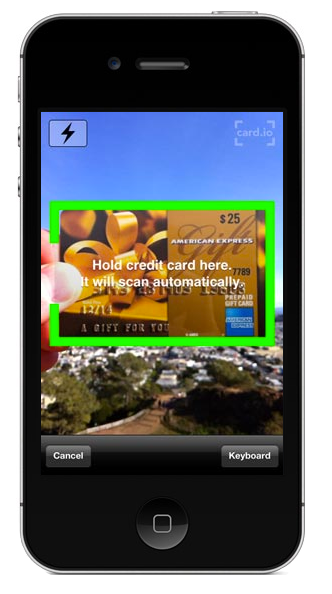
\includegraphics[width=6cm]{cardio}
\caption{Card-io in use sanning a credit card \label{cardioscan}}
\end{figure}



\begin{figure}[ht!]
\centering
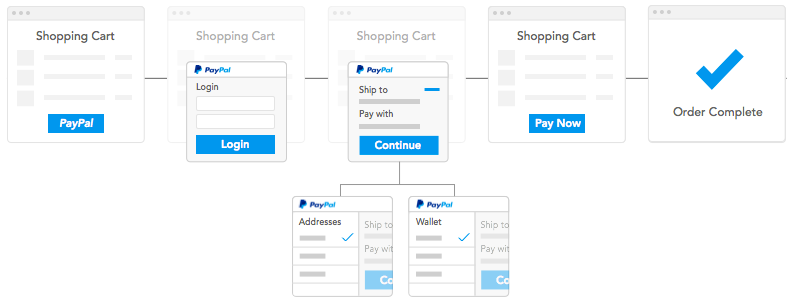
\includegraphics[width=15cm]{vzero}
\caption{PayPal's V.Zero Generic Application Flow \label{vzeroflow}}
\end{figure}

This demonstrates the commercialisation of Douglas' ideas, but this is not the only evolution of reuse, specifically for the personal code reuse of the small-scale developer demographic. However, comparatively less literature has been published and few research efforts made regarding such a demographic, as noted by \cite{Norton2003a} and \cite{Hsieh2006}. The majority of literature refers to large software organisations, but there is considerable need for personal code reuse as well. Norton notes that the majority of small-scale reuse is ad hoc and unstructured, whereas structuring such reuse would enable the developer to become much more efficient with their reuse, and so improve the benefits of engaging with it. The history of such personal reuse, therefore, is difficult to research, but Norton and Min-Sheng both note that there is no obvious practice or standard in place, unlike component-based software engineering.

Therefore, it is clear that code reuse remains a popular concept, and one which can be, and is, employed in multiple ways, dependent on individual ideals; from Douglas' ideas on industrialisation of software development to the current day company repository and work methods, code reuse is ever popular. 

However, small-scale code reuse has been given far less attention, despite it being applicable for individuals throughout their careers, and specifically those that work in relative isolation, such as students, hobbyists, consultants or freelancers \cite{Norton2003a}. Therefore, in the next section, we turn to industry, to seek and analyse potential tools these developers could use that have been built as products instead of research, as well as those available for larger organisations and the industry as a whole.

\section{What tools are there currently that attempt to partially or completely fulfil the goal of cross project, multi user code reuse?}
In this section we will take a look at existing technologies related to the problem domain and analyse their functionality. At the end of the section, we list a set of features these tools may possess, related to fulfilling the original problem description set out in chapter 2, and examine how completely the tools fulfil these requirements.

The technologies below were chosen for a number of reasons, including the author's knowledge of the industry and code reuse, google searches for code reuse tools and similar keywords, and popular technologies. For example, git and GitHub are industry-standard project repositories and implement sophisticated version control and project management tools, so git was chosen based on its widespread use and popularity.

In contrast, Snipplr was found from a search on google using key words “code snippet reuse tool”, and was selected on its immediate similarity to the author's suspected final solution, however, further analysis would reveal that several key features are missing. Finally, the author of this dissertation has experience with several of the tools listed, such as Stack Overflow, and so these tools were included as potential solutions in need of further analysis.

The technologies are presented in ascending order of the author's perceived 'fit for solution', beginning with those which least fit the author's imagined ideal solution. This ideal solution draws from a number of aspects, including the author's personal experience with code reuse, the literature discussed earlier within this chapter and in hindsight of the below complete analysis of the listed technologies. We begin with a minimalist code paste tool, Codepad.org.

\textbf{A} - \textit{Codepad.org} is an online compiler/interpreter that has paste dump capabilities. It allows users to type or paste code from one of 12 languages in to a multiline text box, and then it runs that code and outputs a short URL containing both the source code and any runtime output, which can then be shared by the end user. It is a minimalist code share tool, where source can be saved as 'pastes', and shared via URL. There is little other functionality, other than the ability to make a paste private or save a paste to your account.

\textbf{B} - \textit{Pastebin.com} is similar to Codepad, in that it facilitates 'copy paste' code sharing via a short URL, but does not run the code. It was created in 2002, but was not a popular platform until 2010, when it had achieved 1 million 'active' pastes \cite{Kumparak2011}. In June 2015 this number was more than 65 million active pastes. Pastebin contains more options than Codepad such as language specific syntax highlighting, paste expiration settings, public or private pastes as well as giving it a title, but again does not expand further than simply 'code paste' sharing. Pastebin also exposes an API to allow other tools to utilise its method of sharing, though most seem to be browser plugins. These can be seen on the pastebin website, under tools.

\textbf{C} - \textit{Google Docs} allows users to create and edit documents online, including text documents, spreadsheets, slideshows and forms. It originated when Google acquired Upstartle in 2006 and through 2007 merged their web-based word processor with Google Spreadsheets \cite{Mazzon2006}. While not specific to code, it boasts good online, collaborative features for editing documents, as well as cloud storage, and the ability to make documents private, public shareable or public editable. It also includes version history and roll backs for version control. Despite these features, it is not designed for code storage or retrieval. Retrieving code from the storage would quickly become cumbersome as no efficient categorisation or search tools are present, and performance is on par with NTFS. Therefore, Google Docs' main appeal is real time collaboration and version control of documents.

\textbf{D} - \textit{Stack Overflow} is a language-independent, collaboratively edited question and answer website, and contains a vast wealth of knowledge, and often examples too. It began in 2008 as a website dedicated to helping users seek assistance on programming related issues. Soon after in 2009, additional websites were created along the same premise, under the Stack Exchange umbrella. Within Stack Overflow, questions and answers are voted up and down, and edited in the same fashion as a wiki. Reputation is gained or lost from these votes, resulting in self-policing and consistent high quality content. These features relate to the problem domain as they help reduce stale code, and provide peer review for code snippets. They also allow editing of answers as programming languages evolve and standards change, which is something a static repository often fails to achieve. However, as it is a question and answer website, code sharing is reactive, and usually occurs as an example within an answer. It most certainly does not act as an adequate repository, despite its many usability and collaborative features. Despite this, it is worth noting for its usability features, as discussed.

\textbf{E} - \textit{Integrated Development Environments} (IDE) may come with snippet tools. Sublime and Atom are both text editors for code and markup that include some form of snippet repository within them. These are offline, personal repositories, but the specific files can be zipped and sent to others, albeit with effort from both parties. The snippets are written and stored as files with some form of markup, for example XML. This then allows them to be named, and recalled simply by writing the name of the snippet. For code that is used often, this is a fast and efficient way to reuse code, but requires the developer remember both what snippets are available, and what name they all go by. Searching the repository is often cumbersome, and redundancy is quite possible, as snippets may go forgotten. As it is an offline, personal repository, the problems relating to stale code and lack of peer review remain.

IDE Plugins are also an option, such as Resharper for Visual Studio. Its aim is to improve upon Visual Studio's snippets, though works in quite the same way as the IDE snippet tools mentioned above. Resharper however, can also predict which snippets you may want from the context of your code, among other things. Despite this functionality, it again is an offline, personal repository and maintains the same problems mentioned above that befall the IDE solutions.

\textbf{F} - \textit{git} is a version control software, storing revisions of software in a distributed revision control system, and is widely used in the software development industry \cite{Skerrett2014}. Users can create a repository which maintains a complete history and full version-tracking of itself. This repository can then be cloned to another location to be worked on, and this second repository also maintains a complete history and full version-tracking. Commits can then be pushed between repositories, and changes are merged to allow for seamless collaboration even on the same files. However, git repositories mirror that of a file system, and as such have no real search or sort methods to allow for quick navigation through code snippets. Instead they are used to track source code for individual projects. This would make it cumbersome to use, and although it improves on Google Docs, as it is code oriented, it does not satisfy the ease of access nature that a code reuse repository would require.

\textbf{G} - \textit{GitHub's Gists} initially look very similar to pastebin and codepad, in that the user may type or paste a snippet of code into a textarea, giving it a title, description and privacy options, and then share it via a URL with other users. However, once created, they are treated as a git repository, and can be cloned, revised and added to. This means they act as a combined pastebin and git, bringing with it the benefits of both, however this solution does not improve on the negative points mentioned above for either, and so again would not be suitable as a solution to the problem at hand.

\textbf{H} - \textit{Codebase} is an online repository hosting service that works with git and other similar repository services, but with project tracking features on top. Similarly, Codebase is used to track source code for individual projects, and also handles a number of other project management features, such as tickets, bug tracking, time tracking, customisable permissions, AGILE development and more. A number of these features would be useful in our ideal solution, however again Codebase falls short as it is cumbersome to extract snippets from a repository built in this manner. 

\textbf{I} - \textit{Snipplr} is an online snippet sharing website, and comes close to solving the problem. Users can create public or private (personal) snippets, containing a title, description, source code and other meta data, and save them to their own snippet library. If public, other users can comment on these snippets, favourite them or share them on social media. Snipplr has a number of search filters, including searching all snippets or just personal snippets, searching titles and descriptions, searching source or for specific tags. However, the search functionality is particularly verbose, and only allows for searching one of these filters at any time. Combination search is impossible, so complex filters cannot be created.
Users have profiles, and can gain points and achievements for their snippets through community recognition, in a similar fashion to StackOverflow, and high scoring snippets are more visible to the community. Users also can edit their own profiles to provide personal information about themselves.

At first look Snipplr seems to fit the bill for our problem domain, but a number of features are lacking. There is no version control or snapshot history for code snippets, and by extension there is no tracking information other than time and user of last edit. Additionally, Snipplr has no functionality geared towards sharing within a company or institution. If a company, such as a web development agency, wished to track reusable snippets and provide access to a list of employees, there is no process to do this with Snipplr. Similarly, if an educational institution wished to share code snippets with a specific subset of students, Snipplr would be unable to handle this request. Therefore, a comparison of these core features are necessary, to find which, if any, are most suited as our solution.

\section{What core features can we draw from these tools for our ideal solution?}
From the above break down of these technologies, we can establish preliminary criteria drawn from these tools that we believe would benefit the small scale code reusers. These criteria also allow us to both compare the tools with each other, and begin to conceptualise an ideal overall tool that consists of these criteria. Finally, it allows us to see if any one technology already fits in to this ideal overall tool, or how closely any one technology comes.

Table \ref{corefeatures}. culminates this information, with the individual technologies along the top and the criteria on the left. If the technology implements the criterion listed, a checkmark is placed in the corresponding box.

Before displaying the table, it is useful to explain the chosen criteria, to help give an understanding and greater depth to each criterion. The following bulleted list details this information:

\begin{itemize}
\item \textit{Paste Dump} - Some functionality specifically designed to allow writing or pasting code into a multiline text field, and the ability to find that code again via a URL. 
\item \textit{Exposed API} - An API that enables some or all of the technology to function through third party code, such as calling savePaste(string) or getPaste(id) for a paste dump.
\item \textit{Publicity Settings} - Some functionality that enables some or all of a user's input to be set to public or private. See Grouping Privacy criterion for explicit settings.
\item \textit{Openly Collaborative} - The technology provides the ability for multiple users to collaborate on a single, shared input to the technology. 
\item \textit{Online} - The tool can be accessed over the web, independent of device. Does not exclude the possibility of the tool also functioning offline.
\item \textit{Peer Review} - The ability for other users to view and comment on a piece of code. Functionality could be extended to allow for change requests to be sent, or actual changes to be made by users.
\item \textit{Advanced Search/Sort} - The technology provides advanced search and sort capabilities, including complex filters and search terms such as wildcards, to build a complete search term. 
\item \textit{Version Control} - The technology has some form of version control, including a revision history, accountability tracking and the ability to access the previous versions of the code. 
\item \textit{Grouping Privacy} - The technology provides features that allow groups of people to be defined, and for those groups to be given access to specific portions of the stored code, such as an institution giving private code to its members.
\item \textit{Personal Repository} - The technology provides a personal repository for the users, such as an individual area with space for the user to store what they desire.
\item \textit{Not project focused} - The technology does not focus on projects or project management, and instead remains more abstract.
\item \textit{Snippet Meta Data} - Inputs can be attributed with meta data, such as title, description, search tags, etc.
\item \textit{Synchronisation across devices} - The inputs are synchronised across devices, so changes made on one system are reflected on the others.
\item \textit{Accountability} - Any input, be it an addition, change or deletion, can be attributed to a user, and no such action can be performed anonymously.
\end{itemize}

These criteria were chosen from the set of core features implemented by the previously mentioned technologies, and were selected due to their likely utility within a final code reuse tool. The table below summarises these tools based on these criteria, and we shall use this as our main comparison between the tools. The letters and their corresponding technologies are repeated beneath the table for clarity.


\begin{table}[H]
\centering
\caption{Comparison of core features between existing technologies \label{corefeatures}}

\begin{tabular}{|l|*{9}{c|}}
\hline
                                     & A & B & C & D & E & F & G & H & I \\ \hline
Paste Dump                 & \ding{51} & \ding{51} & & & & & \ding{51} & & \\ \hline
Exposed API                & & \ding{51} & \ding{51} & \ding{51} & \ding{51} & \ding{51} & \ding{51} & \ding{51} & \ding{51} \\ \hline
Publicity Settings          & \ding{51} & \ding{51} & \ding{51} & &  & \ding{51} & \ding{51} & \ding{51} & \ding{51} \\ \hline
Openly Collaborative    & &  & \ding{51} & \ding{51} &  & \ding{51} & \ding{51} & \ding{51} & \ding{51} \\ \hline
Online & \ding{51}     	  & \ding{51} & \ding{51} & \ding{51} &  & \ding{51} & \ding{51} & \ding{51} & \ding{51} \\ \hline
Peer Review                 & & & & \ding{51} & & \ding{51} & \ding{51} & \ding{51} & \ding{51} \\ \hline
Advanced Search/Sort & & & & \ding{51} & & & & & \\ \hline
Version Control            & & & \ding{51} & \ding{51} & \ding{51} & \ding{51} & \ding{51} & \ding{51} & \\ \hline
Grouping Privacy         & & & \ding{51} & & & \ding{51} & & \ding{51} & \\ \hline
Personal Repository    & & & \ding{51} & & \ding{51} & \ding{51} & \ding{51} & \ding{51} & \ding{51} \\ \hline
Not Project Focused    & \ding{51} & \ding{51} & \ding{51} & \ding{51} & \ding{51} & & & & \ding{51} \\ \hline
Snippet Meta Data       & & \ding{51} & & \ding{51} & \ding{51} & \ding{51} & \ding{51} & \ding{51} & \ding{51} \\ \hline
Sync Across Devices   & \ding{51} & \ding{51} & \ding{51} & \ding{51} & & \ding{51} &  & \ding{51} & \ding{51} \\ \hline 
Accountability              &    &    &    & \ding{51} &     & \ding{51}  &      & \ding{51} & \ding{51} \\ \hline \hline
\textbf{Total Checks}   & 5 & 7 & 9 & 10            & 5  & 11            & 10 & 10           & 10 \\ \hline
\end{tabular}
\end{table}

\begin{enumerate}[label=\Alph*]
\item - \textit{Codepad}
\item - \textit{Pastebin}
\item - \textit{Google Docs}
\item - \textit{Stack Overflow}
\item - \textit{IDE \& Plugins}
\item - \textit{git}
\item - \textit{GitHub Gists}
\item - \textit{Codebase}
\item - \textit{Snipplr}
\end{enumerate}


These criteria are necessary in order to evaluate and compare the systems, but they will also provide a base from which to advance future research from, specifically in the next chapter when we question current industry experts for their habits and ideals behind code reuse at this scale. 

The criteria table shows us a number of important facts, as well as which technologies stand out as most matching our ideal set of criteria. We can see that codepad and pastebin are part of only three technologies that incorporate a paste dump, and that Gists is the only tool that acts further upon these paste dumps, turning them into repositories of their own to be worked on further. We also see that being \textit{Online} and having an \textit{Exposed API} are common attributes, appearing in all but one of the technologies. This would suggest that online tools are preferred, either by the developers to build or the users to utilise, though this may also be due in part to the research methods utilised and so needs further research to fully justify the reasoning.

It is clear that the paste dump services and the IDE \& Plugins do not facilitate the role of a code reuse repository akin to the likes we are looking for. They each meet half or less of the criteria, and implement no advanced features (such as version control or advanced search/sort). However, their functionality is not implemented by the majority of the other technologies. This makes them worth reviewing as we will need to analyse whether that functionality is necessary in our final application, why other technologies haven't replicated the functionality, and whether their API is worth using instead if that functionality is required. We can see that GitHub's Gist ties in their paste dump service with the other features, and so this will be the system we analyse further when we look to develop or implement paste dump functionality.

\textit{Publicity settings and Snippet Meta Data} are two more features commonly seen throughout our chosen technologies. Each were seen in seven of the nine technologies, suggesting they are also key features of the technology. Publicity settings did not appear in the IDE \& Plugins or on Stack Overflow, though this is likely due to the nature of the two technologies - the IDE \& Plugins were offline and specifically designed for one person, so would not need publicity settings, and Stack Overflow, being a collaborative Q\&A system, would not function with publicity settings. It would, however, be possible for Stack Overflow to implement a group privacy setting to restrict certain questions from only being answered by set groups, though this is not something I witnessed.

\textit{Group privacy}, instead, is implemented by a subset of the technologies which implemented publicity settings, by only Google Docs, git, Gists and Codebase. The author of this dissertation feels this feature is important when considering functionality of the envisioned system, as it would allow for groups or institutions to utilise the technology and restrict access to only its members. This feature is one of several which Snipplr do not implement, along with version control and advanced searching and sorting, which are key reasons why Snipplr does not fully encompass the expected outcome deliverable of this dissertation.

Of these final other features, \textit{Version Control} is the more common, being seen in 6 of the technologies, however, advanced searching and sorting can only be found in Stack Overflow. For a repository, being able to search for complex terms and filters efficiently is a key requirement to facilitate the reuse of deposited code, and aid the user in finding code they may not know exists within the repository. This is because users of the repository must be able to find and reuse components faster and easier than writing the code from scratch \cite{Krueger1992}. 

Human beings are utility-maximizers \cite{Cognition1997} - that is to say, they seek the approach that yields more value than its cost, meaning code reuse will only be embraced when it is believed that reusing the code is easier than writing it themselves. Users may remember a piece of code, but not when or for what they developed it, which makes finding and reusing the code difficult or more cumbersome. A reuse repository requires that finding and reusing the code be more efficient than simply rewriting it, which in turn requires that searching the repository be fast and efficient. If one must spend 10 minutes recalling the code, and another 10 searching for it, when it could have been written in 15 minutes, the repository is not fit for purpose and instead negatively impacts the developer. To this end, advanced searching and sorting is a key component of the ideal solution, and therefore, the technologies that do not implement this feature are far less likely to fully encompass the requirements of our expected deliverable. Consequently, we shall focus on Stack Overflow when we research further into advanced search and sorting, to identify how it should be implemented in the final deliverable.

We have discussed the core features of these technologies and explained the reasons behind why they are important. This has shown that no single technology fully encompasses these requirements despite their relevancy in the final deliverable, and would suggest that the final deliverable itself will be a new technology, built from the core criteria researched above.

Having established these core criteria for our system, we can now begin to look at optional features that the existing technologies implement - usability features that aren't necessary for full functionality, but that improve the day to day usage of these specific tools. In the next section, we discuss the most prominent usability features pulled from our set of technologies, and evaluate how each tool improves the quality of the software and its use.

\section{What usability features do these tools implement and utilise?}
The discussed technologies implement a large array of usability features, ranging from user interface additions or backend functionality, to user-to-user interaction or organisation tools. For this reason, noteworthy features have been extracted from the technologies and grouped in to categories, then given a brief description to aid understanding. The categories were chosen by the author in an attempt to encompass fully the selected optional features, and provide a logical categorising for analysis.

\begin{itemize} 
	\item User Interface
	\begin{itemize} 
		\item Markdown for description or comments
		\begin{itemize}
			\item Utilises plain text formatting syntax to mark-up text, to be easily translated into HTML and other formats for display. \cite{Markdown2004}
		\end{itemize}
		\item WYSIWYG Text Editor
		\begin{itemize}
			\item What You See Is What You Get - allows the developer to see what the end result will look like while the source is being written \cite{Oxfordnd}, such as when HTML or Markdown is included in the text.
		\end{itemize}
		\item Syntax Highlighting
		\begin{itemize}
			\item Changes the colour of text, usually source code, according to a catalogue of terms or a language syntax, such that the readability is improved.
		\end{itemize}
	\end{itemize}

	\item User-to-User Interaction
	\begin{itemize}
		\item Rate, Pin/Favourite, Comment, Share
		\begin{itemize}
			\item Ratings allow users to express their opinions quickly and show the aggregate opinions of fellow users, for example through a 5 star rating, or by giving users the ability to +1 or -1 the score of a submission.
			\item Pining or Favouriting is the act of a user expressing their want to return to the submission for future use by storing it in a special, personal list.
			\item Commenting goes further than rating, by giving the user a way to express their opinion verbatim, and culture discussion around a submission.
			\item Sharing allows users to bring others into the fold by distributing the submission, through social media or more conventional methods such as email.

		\end{itemize}
		\item Profile - information about the user, their submitted code and more
		\begin{itemize}
			\item The profile allows a user to find out more about other users, or look at other user's submissions to the technology.
		\end{itemize}
		\item Achievements
		\begin{itemize}
			\item Achievements are a method of gamification \cite{Huotari2012} for a technology, and promote user activity through unlocking rewards for completing tasks.
		\end{itemize}
		\item Report Submissions
		\begin{itemize}
			\item This allows for a community to self-police itself, and ensure unwanted or spammy posts are removed with less or minimal effort.
		\end{itemize}
	\end{itemize}

	\item Content Navigation
	\begin{itemize}
		\item Tagging, Indexing, Searching/Sorting
		\begin{itemize}
			\item Tagging allows users to add specific meta data to submissions to aid future search and sorting. This could involve describing the type of submission, where or when it was written, or what language it's in, and is commonly seen as a list of key words. 
		\end{itemize}
		\item User groups/companies/institutions
		\begin{itemize}
			\item The technology enables users to create groups and invite other users in to them. They may have a hierarchy of admins and members, or have all users be equivalent, and can be used by companies or institutions to distribute submissions to all of its members.
		\end{itemize}
		\item Public/Private snippets/groups
		\begin{itemize}
			\item The ability to mark a submissions as public or private, or add a list of users that are able to view the submission, either individually or as a group.
		\end{itemize}
		\item Forks/Change Requests/Branches
		\begin{itemize}
			\item Users are able to take a copy of a submission and change it, potentially submitting their own, or requesting that the original one be merged or replaced with their updated version.
		\end{itemize}
		\item Related submission
		\begin{itemize}
			\item The technology provides quick access to related submissions that the reader may be interested in viewing or using.
		\end{itemize}
		\item Submission Grouping/Multi-part Submission
		\begin{itemize}
			\item The ability to create submissions that are part of a small collective of submissions, and as such are linked together by some method.
			\item For example, a submission may be for template code for a dynamic button on a website. One part utilises HTML for markup, another uses CSS for styling and a third part incorporates JavaScript for animation.
		\end{itemize}
		\item Custom groups for submissions
		\begin{itemize}
			\item Predefined or User-created groups for submissions, such as collecting snippets used in web development, those used in software development, and design documents all into different groups for ease of access.
		\end{itemize}
		\item Cloud Storage/Computing
		\begin{itemize}
			\item Cloud Computing refers to on-demand network access to a set of resources, often utilised as programs that don't need to be downloaded, installed or run on the local system \cite{Anjomshoaa2011}.
			\item Cloud Storage refers to data being stored across multiple servers or locations, with the digital representation of this data exists in a single access point for use, such as on one website.
			\item This allows for applications to be used immediately, from any host, without any prerequisite short of internet access and some medium, such as a browser, making it highly accessible.
		\end{itemize}
	\end{itemize}

	\item Third party tools

	\begin{itemize} 
		\item Integrated Development Environment (IDE) Integration via API
		\begin{itemize}
			\item Snippets saved to the technology can be accessed from within the IDE via exposed hooks to the technology. Might include user authentication.
		\end{itemize}
		\item Facebook Login for easy account creation/future login
		\begin{itemize}
			\item Utilising exposed account APIs via OAuth protocols, user details can be passed from Facebook to the technology to facilitate account creation and login.
		\end{itemize}
		\item Social Media integration for sharing code
		\begin{itemize}
			\item Exposed API from social media allows code to be shared on those social media, such as Tweets on Twitter or Facebook messages.
		\end{itemize}
		\item WordPress Plugin
		\begin{itemize}
			\item Similar to social media integration, a WordPress plugin would allow functionality from the website to be utilised by the WordPress platform, and as such, by websites running WordPress.
		\end{itemize}
	\end{itemize}
\end{itemize}

These usability features are all optional for a final system, but each one can be useful for specific use cases or certain user bases. For example, \textit{Third Party Tools} enable the technology to fit more easily in to a user's workflow, or create a more seamless integration for utilising the tool, including before, during and after development, such as planning, developing and sharing. \textit{User Interface} additions help make the technology more accessible, efficient or easier to use, and can help users quickly understand how to use the technology, or make sense of a submission, such as with Syntax Highlighting.

\textit{User-to-user interaction} is important to promote a social environment within the technology, while also enabling users to more easily engage in cross-user interaction. User interaction facilitates two of the core features, collaboration and peer review, and as such, these optional features play an important role in the final system. Finally, \textit{Content Navigation} makes up a large bulk of the optional features, which is to be expected, as the technology will be responsible for storing, categorising and retrieving content in the form of submissions and as such, these features will focus heavily throughout the technology.

The next step for the optional features is to describe their priority relative to each other. In the next chapter, we delve into this task, and present opinions collected from an array of end users, including industry professionals from a range of companies, and undergraduate students studying Computer Science. Ultimately, we intend to finalise the requirements for the deliverable.

\section{Conclusions}
As stated at the start of this chapter, our goal throughout this section was to determine whether the problem domain of small scale code reuse has been sufficiently explored, and whether there are adequate technologies currently that address the domain. We explored the history of code reuse, from its roots up to its modern day evolution, and discovered that, although papers on reuse are not uncommon, those focused on individual or small scale reuse are sparse, and this has been noted in several published works.

We also described nine potential technologies, and investigated how they work and what they accomplish. From this we identified fourteen core criteria that our desired system should facilitate. Unfortunately, none of the technologies managed to fully encompass all these requirements, which suggested that technology, like the literature, does not provide adequate coverage for users of small scale code reuse. 

Further to the core features, we identified many optional features that promote user experience. These were aggregated from the technologies we described, and will be used in practical research to help mould the deliverable we intend to create. This practical research will be conducted with the help of professionals from multiple industries, and students in educational institutions. We will utilise their input and knowledge from their own code reuse experiences, and collaborate their feedback and opinions into the requirements and design phase throughout the next chapter.

To conclude, we feel there has not been adequate research in to small scale code reuse, nor is there a sufficient technology able to fully address the needs of the code reuser. We intend to design, construct and evaluate such a technology in an open source environment, with the desire of improving small scale, cross project code reuse. The first step for this begins in our next chapter: the requirements and design for such a system.




%% Chapter for the Requirements and Design
\chapter{Requirements \& Design}
%% If you are doing a primarily software development project, this is the 
%% chapter in which you review the requirements decisions and
%% critique the requirements process. Then, you review your design decisions at various
%% levels and critique the design process.

\section{Introduction}
Throughout this chapter, we detail the requirements for our system, both functional and non-functional, by drawing on the core and optional features described in the previous chapter. With these in mind, we then move on to consider the design of our proposed deliverable, and set specific goals for it, which will later be used as measurements of evaluation for the system.

\section{Requirements}
We begin by translating the previous core features in to functional and non-functional requirements, 



\chapter{Implementation \& Testing}
This is the chapter in which you review the implementation and testing
decisions and issues, and critique these processes.


\chapter{Evaluation}
This is the chapter in which you review the outcomes, and
critique the outcomes process.  You may include user evaluation here
too.

Code can be output inline using \verb@\lstinline|some code|@.  For example,
this code is inline: \lstinline|public static int example = 0;|  (I have
used the character \verb@|@ as a delimiter, but any non-reserved character
not in the code text can be used.)

Code snippets can be output using the \verb|\begin{lstlisting} ... \end{lstlisting}|
environment with the code given in the environment.  For
example, consider listing \ref{Example-Code}, below.

\begin{lstlisting}[breaklines,breakatwhitespace,caption={Example code},label=Example-Code]
public static void main() {

  System.out.println("Hello World");

}
\end{lstlisting}

Code listings are produced using the package ``Listings''.  This has many
useful options, so have a look at the package documentation for further
ideas.


\chapter{Results \& Analysis}
This is the chapter where you review your results and analyse them.


%%
%% Now we are back to the standard project contents that you should include
%%

\chapter{Conclusions \& Discussion}
%% Uncomment this to include a separate tex file wih the conclusion contents
%\include{conclusion.tex}

This is the chapter in which you review the major achievements in the
light of your original objectives, critique the process, critique your
own learning and identify possible future work.


\bibliography{BibFile}


\appendix

%%
%% Use the appendix for major chunks of detailed work, such as these. Tailor
%% these to your own requirements
%%

\chapter{Design Diagrams}

\chapter{User Documentation}

\chapter{Raw results output}

\chapter{Code}

%%
%% NOTE that for this to typeset correctly, ensure you use the pdflatex
%%      command in preference to the latex command.  If you do not have
%%      the pdflatex command, you will need to remove the landscape and
%%      multicols tags and just make do with single column listing output
%%

\begin{landscape}
\begin{multicols}{2}
\section{File: yourCodeFile.java}
\lstinputlisting[basicstyle=\scriptsize]{yourCodeFile.java}
\end{multicols}
\end{landscape}

\end{document}
